\chapter{Landauer at the transistor gate: CMOS and the Dennard wall}\label{ch:cmos}

\section{The floor for logic}

A conventional logic gate erases information at almost every operation. The Landauer floor~\cite{Landauer1961} at
a junction temperature $T_j=348$~K (75~$^\circ$C) is
\begin{equation}
 \kB T_j\ln2=3.33\times10^{-21}\ \mathrm J=0.021\ \mathrm{eV}.
\end{equation}
The chip gauge (Chapter~\ref{ch:ascoreqc}) uses whole-chip power divided by transistor count and clock,
$E_{\mathrm{sw}}=\mathrm{TDP}/(N_{\mathrm{trans}}f)$. For the AMD Ryzen~9 9950X (default TDP 170~W, base clock 4.3~GHz~\cite{AMD9950X};
$20.6\times10^9$ transistors in two compute dies and an I/O die) this gives $E_{\mathrm{sw}}=1.92\times10^{-18}$~J per transistor per cycle,
576 times $\kB T_j\ln2$, or $M=E_{\mathrm{sw}}/\kB T_j=399$ (Chapter~\ref{ch:iams_law}) \calc. Most transistors do not switch every cycle,
which raises the energy per actual switch, while TDP also contains leakage and static power, which lowers it; the reading is an
order-of-magnitude figure for the whole chip. The transistor count is the least certain input: it is AMD's launch figure and is not on the
maker's product page \openprob. Present logic therefore runs a few hundred $\kB T$ above the thermal noise quantum per
switch on this average. This is the regime in which thermal physics, not lithography, sets the rules.

\section{Dennard scaling and its end}

Dennard \emph{et al.}\ showed in 1974 that shrinking all dimensions and the supply voltage by
$1/\kappa$ keeps power density constant, while delay falls as $1/\kappa$ and density rises
as $\kappa^2$~\cite{Dennard1974}. The rule held until the mid-2000s. It failed because the
supply voltage cannot fall below a few tenths of a volt without leakage becoming prohibitive.
The subthreshold swing of a MOSFET is bounded below by $(\kB T/q)\ln10=60$~mV/decade at
300~K~\cite{Sze2006}, so the threshold voltage cannot be scaled without an exponential rise
in off-current. Once $V$ is held fixed, power density grows as $\kappa^2$
(Figure~\ref{fig:dennard}). Clock frequencies stalled near 2005, and the industry turned to
multicore designs and, later, dark silicon~\cite{Esmaeilzadeh2011}. Koomey's law, the doubling
of computations per joule, slowed from every 1.57 years to about every 2.7 years~\cite{Koomey2011,Koomey2016}.

\begin{keybox}[title={The Dennard wall is a Boltzmann wall}]
The 60~mV/decade limit is $\kB T/q$ times $\ln10$. The end of Dennard scaling is therefore
a statement that switching energies approached a fixed multiple of $\kB T$ at the junction.
That is the regime IAM describes: an encoding surface (the gate channel) at a definite
temperature ($T_j$), with a floor set by $\kB T_j$. The identification is standard device
physics, and IAM's contribution is to place it on the same axis as the horizon and the qubit.
\end{keybox}

\begin{figure}[htbp]\centering
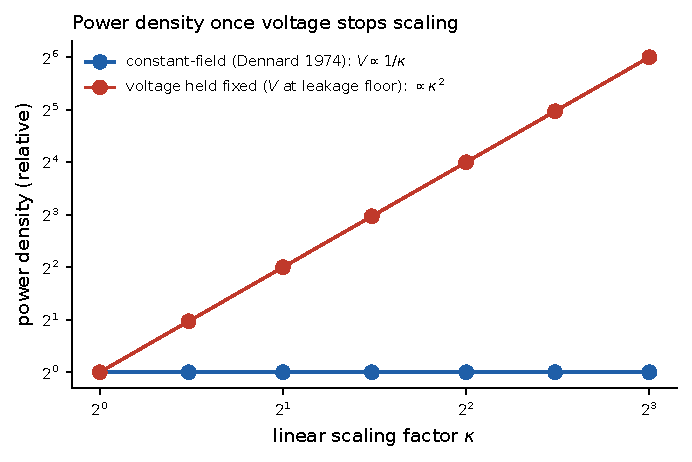
\includegraphics[width=0.7\textwidth]{figures/part3/fig_dennard.pdf}
\caption{Relative power density under constant-field scaling and at fixed voltage.
\derived\ from the 1974 scaling rules.}\label{fig:dennard}
\end{figure}

\section{The chip gauge over time}

Restated on the chip gauge, the history of CMOS efficiency carries three physical observations.
\begin{enumerate}
 \item \textbf{A step series that would cross the floor must end.} The reading cannot fall below the Landauer floor. A constant
       fractional improvement per node, continued, would carry a chip through its own floor in a finite number of nodes; a step size
       that cannot continue must stop. The end of Dennard scaling is where the per-node steps of CMOS efficiency shrank \interp.
 \item \textbf{Temperature response.} Using Eq.~\eqref{eq:npower} in junction temperature, each processor design class carries its own
       exponent $n$; the calibrated values are $n=1.853$ for pre-Dennard CMOS and $0.936$, $0.340$ and $0.794$ for three post-Dennard design
       families \calibrated.
 \item \textbf{Why the exponent is a local slope.} Leakage rises exponentially with $T$, and dynamic energy rises weakly. $n$ is the local
       slope of the mix at the operating point, and it is not derived.
\end{enumerate}

\section{Architecture overhead}

The reading of a chip mixes two components: one set by the process node, which a shrink removes, and one set by the instruction-set
architecture and system design (memory hierarchy, packaging, dedicated accelerators), which no shrink removes. Independent measurements
show that the instruction set itself matters little for energy; the microarchitecture and its implementation dominate~\cite{Blem2013}.
Separating the two components on the chip gauge needs per-block power and activity data from the designs \openprob.

\section{Prediction}

\prediction\ AMD's Zen~6 desktop part on a 2~nm-class process improves on the Ryzen~9 9950X by less than 25\,\%: on the same power (default
TDP) and clock (base) definitions it stays above $0.75\times576=432$ times $\kB T_j\ln2$. Falsified by a step of 25\,\% or more on those
definitions. Chapter~\ref{ch:predictions} (Part~\ref{part:5}) lists it with its test and date.
